\chapter{Method}

Prior to designing the game, background information was collected on developer team's views and expectations on a new Tower Defense game. A number of existing well-known tower defense games were also tested and discussed for research purposes and to get a general idea of what features are desirable. The design process included many discussions of different ideas, drawing of mind maps and sketch-like UML-diagrams.

The development was done in Eclipse IDE with the Android SDK-plugin with the program language Java. Included in Android SDK is an emulator which made it possible to test the code directly on the computer.

The implementation was done using an agile development approach, in the sense that we worked in small iterations and changed the requirements continuously during the development process. To be able to make the project easy to maintain, subversion management with Git was used. This increased our ability to share code within the developer team during the development process, and to allow us to work on multiple parts of the project at the same time. 

%----------------------------------------------------------
\section{Interviews}

Interviews were used as a tool in two different stages of development; the research stage and the final testing stage.

To get a better picture of what makes a Tower Defense game good and try to collecting ideas for the game, interviews were conducted. The interviewees where people that play games regularly and had prior experience of playing Tower Defense games. Ten interviews were conducted, following a unstructured interview template with mainly open questions. The full interview template is found in Appendix APPENDIX"". 

The interviews provided some insight into peoples thoughts and the statements from the participants were used when making important design decisions. It soon became obvious that everyone had their own opinion on which features a good game should include, but several statements were general and helped avoiding common mistakes. 
%----------------------------------------------------------
\section{Git - A version control system}

When developing software in teams, a system to manage and synchronize the source code is needed. This to ensure everyone in the project is working on the latest version of the system. In this project Git was used for this purpose. 

When working with Git each developer included in the project has one local repository on their computer. Changes made to the code is then copied between the other developers local repositories. This does not force the users to have a dedicated server to store a central repository. Instead Git users are free to store their repositories anywhere. (Git, 2010) 

Since Git allows the project to be stored locally on every members computer, work can be done on the implementation despite lack of internet access. This also means that any system failure is only going to affect one individual, who could then fetch an updated version of the project from the other members, providing the project with an increased tolerance to any system breakdowns
%----------------------------------------------------------
\section{Code convention}

Code convention is a huge subject of its own, and it can be divided into subcategories such as style, language and programming practices. When developing a large system it is important to follow a common code style convention. This to make the code easy to understand for other developers that might be working on the system later on. This involves choosing suitable names for variables and classes, as well as making similar choices of code constructions. 

\subsection{Style conventions}

Android is an open source project, and a set of rules have been created to keep a common style between developers. These rules are intended for contributors to the android platform itself. Even though they are not a requirement for application development, they are still well thought out and adapted to the Android environment. For this reason these rules were used as guidelines for this project as well. Some of these could be seen as common sense while others add extra readability beyond what is common in Java programming.

The following are some of the important style conventions that were used, and how they differ from the android contributor rules:

\subsubsection{Javadoc and comments}

Javadoc comments were continuously added to the code, using the standard format as specified in by android. Non-javadoc comments were used as often as well to clearify the code and increase maintainability. A comment including copyright info were not added, since this was deemed to not be needed for the project at this stage.

\subsubsection{Short methods}

Long methods were broken down into shorter ones to increase readability where possible. One good example of this is the method onDraw in the class GameView. This calls several submethods that draws different parts of the game, instead of drawing everything inside one single method.

%--------------------------------
%- Code snippet onDraw
%--------------------------------
\begin{figure}[htb]
\begin{small}
\verbatiminput{code/onDraw.java}
\end{small}
\caption{Caption for onDraw...}
\label{fig:codeExOnDraw}
\end{figure}
%--------------------------------

\subsubsection{Fields}

Fields should either be at the top of the file or immediately before the methods that use them, according to the rules. All fields were declared at the top of the file. Java code conventions recommend field declaration in the following order: "First the public class variables, then the protected, then package level (no access modifier), and then the private." CITE(http://java.sun.com/docs/codeconv/)

\subsubsection{Limit the scope of local variables}

Local variables should be initialized on the same line as they are declared if possible, and also as close as possible to where they are actually used.

\subsubsection{Indentation}

The rules recommend using four spaces instead of tabulations. Since this project was made entirely in Eclipse we chose to use normal tabs. This is the default way to handle indentation when using Eclipse and it is facilitated by using auto-indenting options.

\subsubsection{Field names and other names}

For field names the rules were strictly followed. This means:

%---------------
\begin{itemize}

\item Non-public, non-static field names start with m.
\item Static field names start with s.
\item Other fields start with a lower case letter.
\item Public static final fields (constants) are ALL\_CAPS\_WITH\_UNDERSCORES.

\end{itemize}
%---------------

Additionally field name were carefully chosen so that their purpose was clear, and use of ambiguous names or shortenings was avoided.

\subsubsection{TODO annotation}

The TODO annotation was used extensively during the coding process, to mark unfinished sections in the code. Eclipse automatically recognizes the TODO-comments and makes it even easier for the developer to find them by marking their locations on the scrollbar while browsing the code.

\subsubsection{Logging}

Logging was used for debugging purposes. The log method made it possible to spot sections in the code that was not functional. Debug messages were marked as verbose, meaning that they were only compiled in debug mode. This to ensure that they would not affect the performance of the game.
%----------------------------------------------------------
\section{Android development environment}

Developing standard Android applications requires the Java Development Kit (JDK) and an Integrated Development Environment (IDE). Google recommends Eclipse with Android Development Tools (ADT) for programming applications to Android. The ADT is a plugin for Eclipse allowing easy creation and management of Android projects. CITE HERE""

The Eclipse Foundation is an open-source community originally created by IBM in 2001. Its most popular IDE Package is the Eclipse IDE for Java EE Developers that currently has over 1.2 million downloads. Eclipse IDE is free to use and allows the users to easily create Java applications. (Eclipse Foundation, www.eclipse.org, 2010-04-30)

Figure ~\ref{fig:eclipseIDE} shows a screenshot of a project in Eclipse. The left panel shows all the files in the project and the center panel the current open file. At the bottom there is a console showing the status of the different tasks that Eclipse is performing. To the right is an outline of the methods and variables in the current file. This is generated automatically and helps the user easily overview and navigate the code.

%-------
%- Image eclipse
%-------
\begin{figure}[here]
\begin{center}
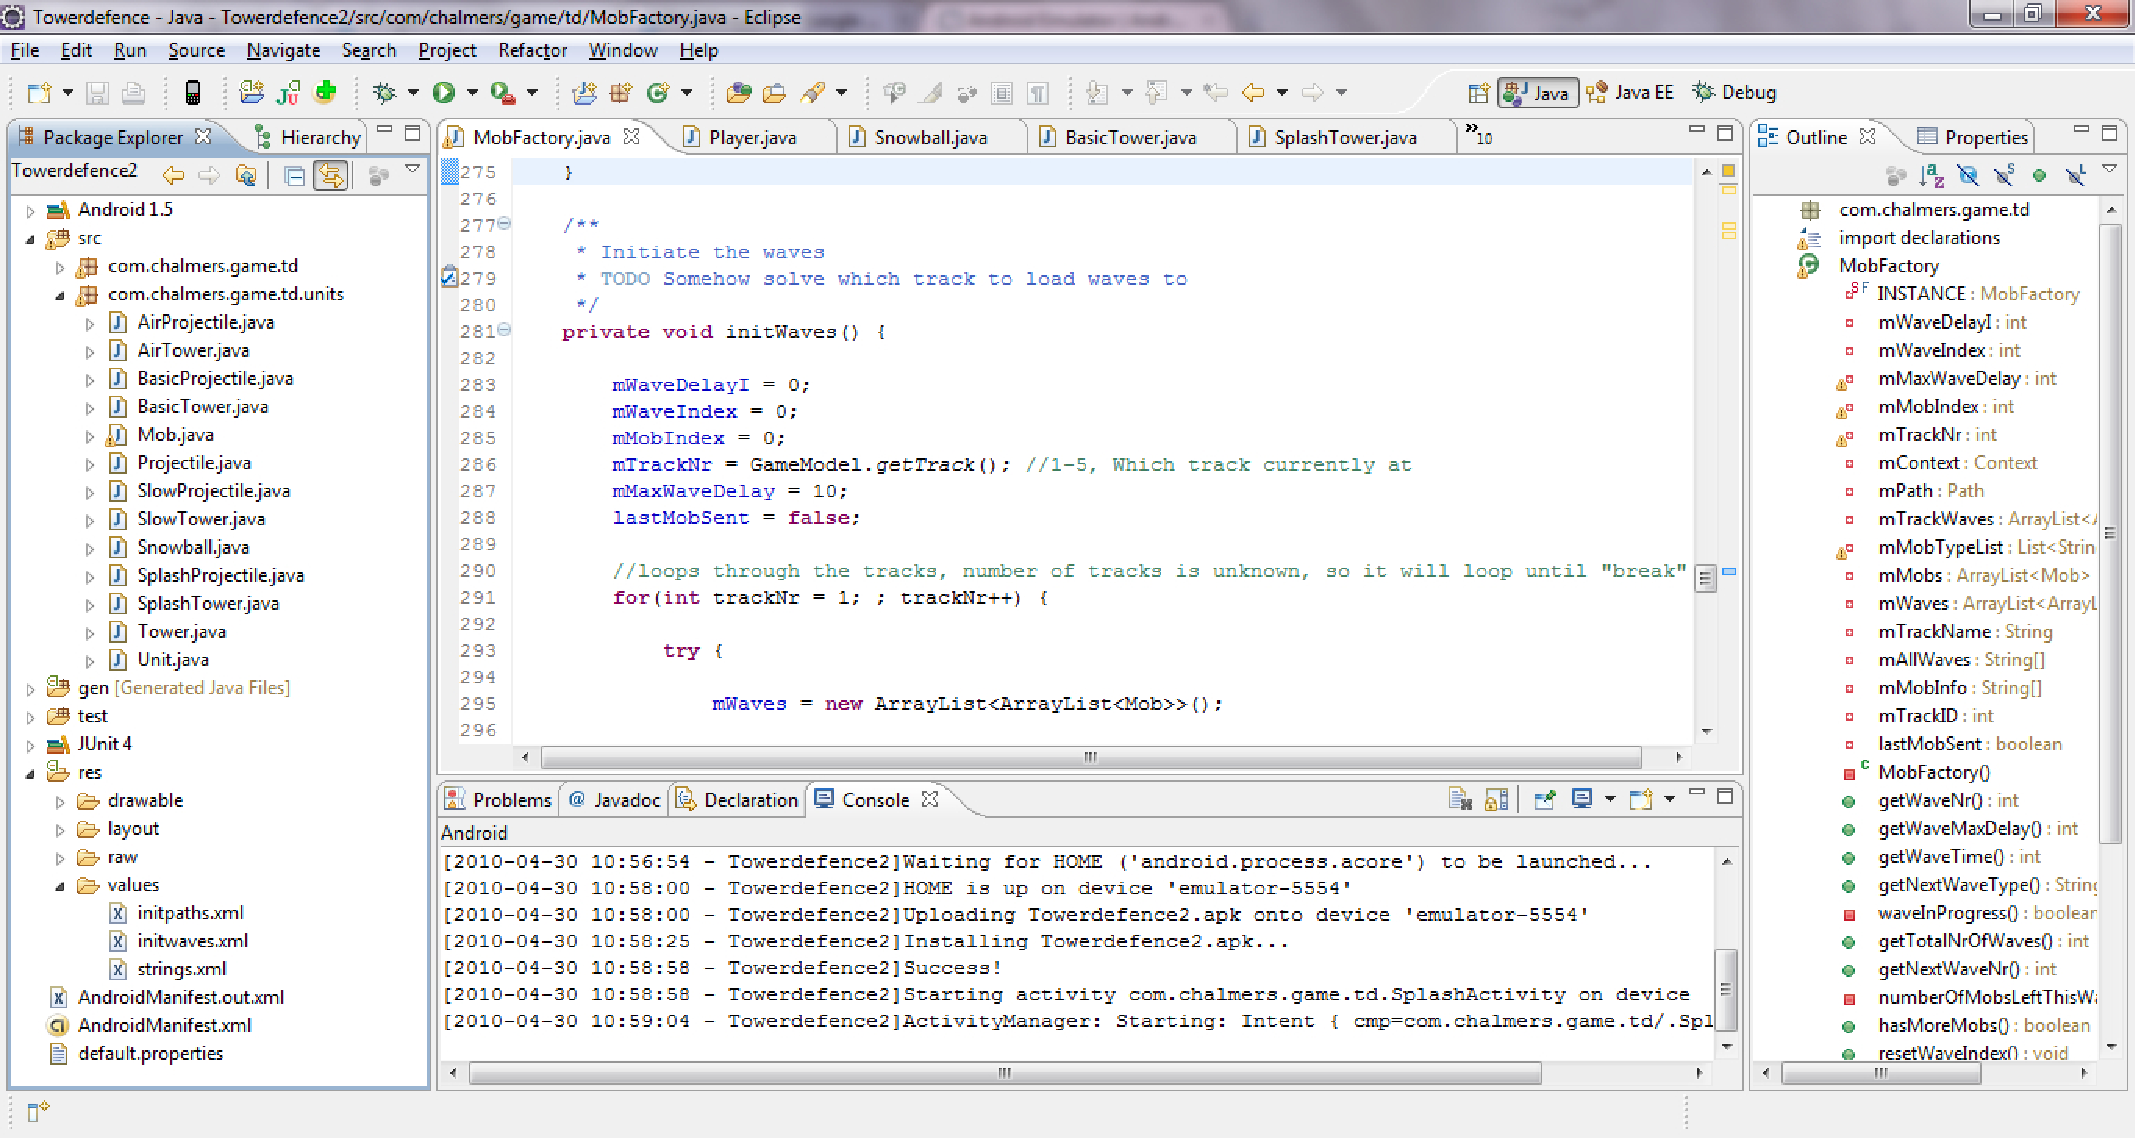
\includegraphics[scale=0.3]{pics/chapters/chapter2/eclipse}
\end{center}
\caption{The eclipse Intergrated Development Environment}
\label{fig:eclipseIDE}
\end{figure}
%-------

The Android Development Kit includes an Android emulator. This allows the developer to test her applications without the use of an actual phone. It supports a majority of the functionalities of a real phone such as simulating SMS, phone calls, events and geographic locations (like GPS navigation). The mouse can be used to click on the screen to emulate usage of the touchscreen of the device. As shown in figure ~\ref{fig:androidEmulator}, there is also access to the buttons normally available on an Android phone. The emulator can be set up to use different versions of Android and different resolutions, allowing the developer to verify compatibility. CITE HERE ""

\clearpage
%-------
%- Image Android emulator
%-------
\begin{figure}[here]
\begin{center}
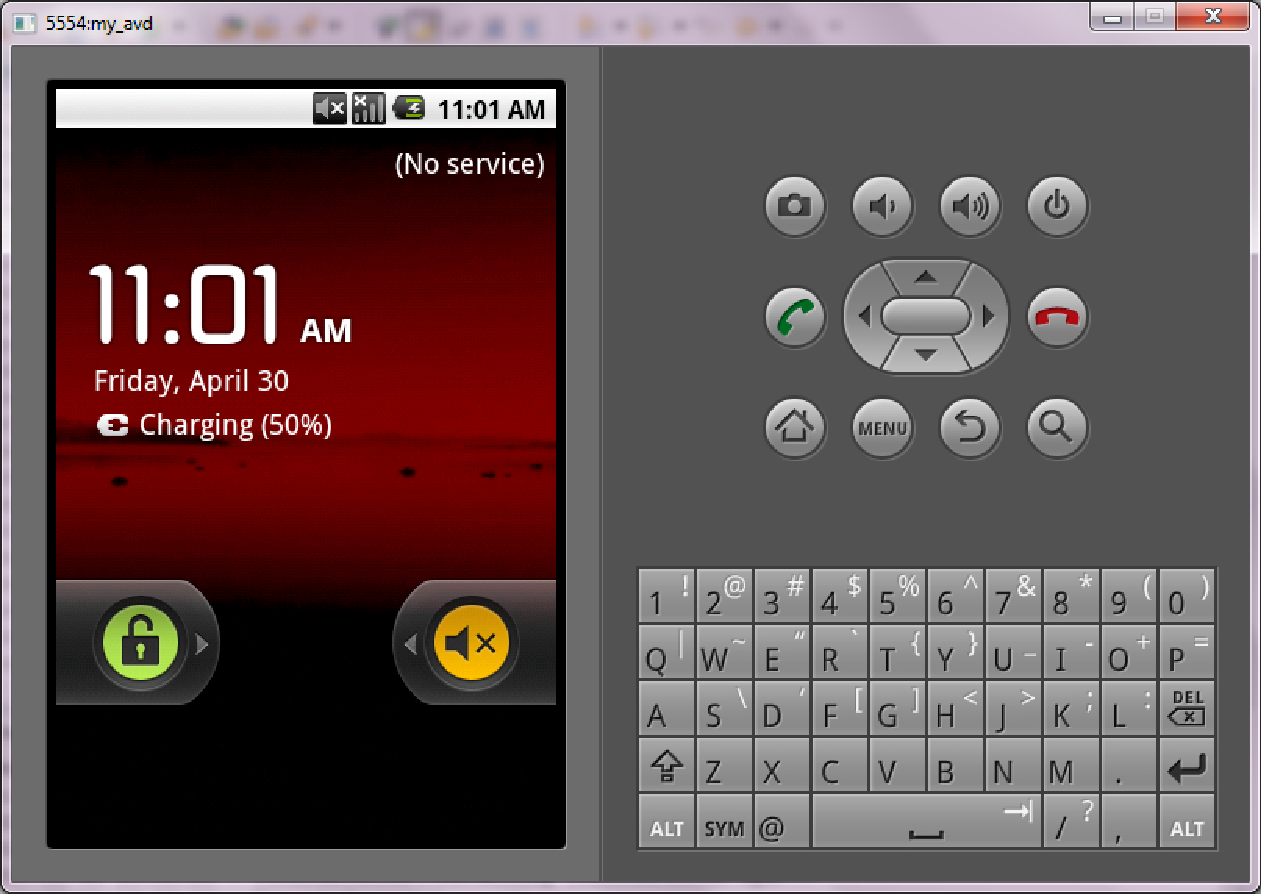
\includegraphics[scale=0.4]{pics/chapters/chapter2/emulator}
\end{center}
\caption{The Android emulator}
\label{fig:androidEmulator}
\end{figure}
%-------